\chapter{Lezione 18}
\label{chap:lezione_18}

\begin{flushright}
\textit{Data: 24/11/2025}
\end{flushright}

\section{Teoria delle Perturbazioni nel Modello di Landau-Ginzburg}

In questa lezione sviluppiamo la teoria delle perturbazioni per il modello di Landau-Ginzburg.
L'obiettivo è calcolare la funzione di correlazione a due punti $G(x)$ espandendo il termine di interazione in potenze della costante di accoppiamento $g$.
Vedremo come i diagrammi di Feynman emergano naturalmente da questa espansione.

\subsubsection{L'Hamiltoniana di Landau-Ginzburg}

Consideriamo l'Hamiltoniana efficace di Landau-Ginzburg. La separiamo in una parte libera (Gaussiana), $\mathcal{H}_0$, e una parte di interazione, $\mathcal{H}_{int}$:

\begin{equation}
    \beta \mathcal{H}[\varphi] = \beta \mathcal{H}_0[\varphi] + \beta \mathcal{H}_{int}[\varphi]
\end{equation}

dove i termini sono definiti come:
\begin{align}
    \beta \mathcal{H}_0[\varphi] &= \int d^D x \left[ \frac{1}{2} (\nabla \varphi(x))^2 + \frac{1}{2} \mu \varphi^2(x) \right] \\
    \beta \mathcal{H}_{int}[\varphi] &= \frac{g}{4!} \int d^D x \, \varphi^4(x)
\end{align}

In questa formulazione, $g$ agisce come parametro perturbativo.
Assumiamo che $g$ sia sufficientemente piccolo da permettere un'espansione in serie di Taylor.

\subsection{La Funzione di Correlazione a Due Punti}

Siamo interessati alla funzione di correlazione a due punti (o funzione di Green):

\begin{equation}
    G(x) = \langle \varphi(x)\varphi(0) \rangle = \frac{\int \mathcal{D}[\varphi] \, \varphi(x)\varphi(0) \, e^{-\beta \mathcal{H}[\varphi]}}{\int \mathcal{D}[\varphi] \, e^{-\beta \mathcal{H}[\varphi]}}
    \label{eq:G_definition}
\end{equation}

Indichiamo la funzione di partizione con $\mathcal{Z} = \int \mathcal{D}[\varphi] e^{-\beta \mathcal{H}}$.
Espandiamo l'esponenziale del termine di interazione:

\begin{equation}
    e^{-\beta \mathcal{H}} = e^{-\beta \mathcal{H}_0} e^{-\frac{g}{4!} \int \varphi^4} = e^{-\beta \mathcal{H}_0} \sum_{n=0}^{\infty} \frac{1}{n!} \left( -\frac{g}{4!} \int d^D y \, \varphi^4(y) \right)^n
\end{equation}

Sostituendo questa espansione nell'equazione \eqref{eq:G_definition}, sia il numeratore che il denominatore diventano serie di potenze in $g$.
Si ottiene la seguente formula generale di espansione:

\begin{tcolorbox}[colback=colorA!10, colframe=colorB!60!colorA,  title=\textbf{Formula di Espansione}]
\begin{equation}
    G(x) = \frac{\sum_{n=0}^\infty \frac{1}{n!} \left(-\frac{g}{4!}\right)^n \int d^D y_1 \dots d^D y_n \, \langle \varphi(x)\varphi(0) \varphi^4(y_1) \dots \varphi^4(y_n) \rangle_0}{\sum_{n=0}^\infty \frac{1}{n!} \left(-\frac{g}{4!}\right)^n \int d^D y_1 \dots d^D y_n \, \langle \varphi^4(y_1) \dots \varphi^4(y_n) \rangle_0}
    \label{eq:expansion_formula}
\end{equation}
\end{tcolorbox}

Qui, $\langle \dots \rangle_0$ indica la media calcolata rispetto alla misura Gaussiana libera:

\begin{equation}
    \langle A \rangle_0 = \frac{\int \mathcal{D}[\varphi] A[\varphi] e^{-\beta \mathcal{H}_0}}{\int \mathcal{D}[\varphi] e^{-\beta \mathcal{H}_0}}
\end{equation}

Ricordiamo che per la teoria Gaussiana ($g=0$), la funzione a due punti è il propagatore libero:

\begin{equation}
    G_0(x) = \langle \varphi(x)\varphi(0) \rangle_0 = \int \frac{d^D k}{(2\pi)^D} \frac{e^{i \vec{k} \cdot \vec{x}}}{k^2 + \mu}
\end{equation}

Nello spazio dei momenti questo propagatore si comporta come $1/k^2$.
Nello spazio reale, ciò implica che i segnali viaggiano a lungo raggio.
Avvicinandoci al punto critico, la massa $\mu \to 0$ (o $m \to 0$), il che implica che la lunghezza di correlazione diverge ($\xi \to \infty$).

\subsubsection{Teorema di Wick}

Per valutare termini della forma $\langle \varphi(x)\varphi(0)\varphi^4(y) \rangle_0$, utilizziamo il \textbf{Teorema di Wick}.
Esso afferma che la media di un prodotto di campi in una teoria Gaussiana è uguale alla somma su tutti i modi possibili e distinti di contrarre i campi a coppie (propagatori).

\begin{equation}
    \langle \varphi(x_1) \dots \varphi(x_{2n}) \rangle_0 = \sum_{\text{pairings}}\quad \prod_{\text{pairs } (i,j)} G_0(x_i - x_j)
\end{equation}

Se il numero di campi è dispari, la media è zero.

\section{Correzione al Primo Ordine ($n=1$)}

Calcoliamo $G(x)$ al primo ordine in $g$.
L'espressione formale è:

\begin{equation}
    G_1(x) = \frac{\langle \varphi(x)\varphi(0) \rangle_0 - \frac{g}{4!} \int d^D y \langle \varphi(x)\varphi(0)\varphi^4(y) \rangle_0}{1 - \frac{g}{4!} \int d^D y \langle \varphi^4(y) \rangle_0} + O(g^2)
    \label{eq:G1_fraction}
\end{equation}

\subsection{Il Numeratore}
Il termine di ordine zero è semplicemente $G_0(x)$.
Il termine del primo ordine coinvolge la contrazione di 6 campi: $\varphi(x), \varphi(0)$ e quattro campi nel punto $y$ :  $\varphi(y)\varphi(y)\varphi(y)\varphi(y)$.

\begin{equation}
    \langle \varphi(x)\varphi(0)\varphi^4(y) \rangle_0
\end{equation}

Esistono due modi topologicamente distinti per contrarre questi campi:

\begin{enumerate}
    \item \textbf{Contributo Disconnesso:}
    Contrarre $\varphi(x)$ con $\varphi(0)$, lasciando $\varphi^4(y)$ a contrarsi con se stesso.
   
    \begin{equation}
        \underbrace{\langle \varphi(x)\varphi(0) \rangle_0}_{G_0(x)} \underbrace{\langle \varphi^4(y) \rangle_0}_{3 G_0^2(0)} = 3 G_0(x) G_0^2(0)
    \end{equation}
    Il fattore 3 deriva dal numero di modi per contrarre $\varphi^4(y)$.
   
    \item \textbf{Contributo Connesso (tadpole graph):}
    Contrarre $\varphi(x)$ con uno dei $\varphi(y)$, e $\varphi(0)$ con un altro $\varphi(y)$. I restanti due $\varphi(y)$ si contraggono tra loro.
   
    \begin{itemize}
        \item Modi per scegliere $\varphi(y)$ da accoppiare a $\varphi(x)$: 4
        \item Modi per scegliere dai restanti 3 $\varphi(y)$ per $\varphi(0)$: 3
        \item I restanti 2 campi si contraggono in 1 modo.
        \item Peso totale: $4 \times 3 = 12$.
    \end{itemize}
    \begin{equation}
        12 \, G_0(x-y) G_0(y-0) G_0(0)
    \end{equation}
\end{enumerate}

Quindi, il numeratore è:

\begin{equation}
    N_1 = G_0(x) - \frac{g}{4!} \int d^D y \left[ 3 G_0(x)G_0^2(0) + 12 G_0(x-y)G_0(y)G_0(0) \right]
\end{equation}

\noindent Ecco la rappresentazione diagrammatica dei contributi al primo ordine. 

% -------------------------------------------------------------------
% FIGURA 1: LISTA COMPLETA DELLE BOLLE E DIAGRAMMI (Dal manoscritto)
% -------------------------------------------------------------------
\begin{figure}[h!]
    \centering
    \begin{tikzpicture}[scale=1.3, 
        vertex/.style={circle, fill=black, inner sep=1.5pt},
        label_node/.style={font=\small, align=left}
    ]

    % --- RIGA 1: Propagatore G0(x) ---
    \node[anchor=east] at (-2, 0) {$G_0(x) \quad \to$};
    
    \draw[thick] (0,0) -- (1.5,0);
    \node[vertex, label=below:\footnotesize $0$] at (0,0) {};
    \node[vertex, label=below:\footnotesize $x$] at (1.5,0) {};

    % --- RIGA 2: Bolla Semplice G0(0) ---
    \begin{scope}[shift={(0, -1.5)}]
        \node[anchor=east] at (-2, 0.3) {$G_0(0) \quad \to$};
        \node[anchor=west] at (2, 0.3) {$G_0(z-z) = G_0(0)$};
        
        \node[vertex, label=below:\footnotesize $z$] (z) at (0.75, 0) {};
        \draw[thick] (z) .. controls (0.2, 0.8) and (1.3, 0.8) .. (z);
    \end{scope}

    % --- RIGA 3: Doppia Bolla (Figure 8) G0^2(0) ---
    \begin{scope}[shift={(0, -3.0)}]
        \node[anchor=east] at (-2, 0) {$G_0^2(0) \quad \to$};
        
        \node[vertex] (z8) at (0.75, 0) {};
        % Loop sopra
        \draw[thick] (z8) .. controls (0.2, 0.8) and (1.3, 0.8) .. (z8);
        % Loop sotto
        \draw[thick] (z8) .. controls (0.2, -0.8) and (1.3, -0.8) .. (z8);
    \end{scope}

    % --- RIGA 4: Diagramma Connesso (Tadpole) ---
    \begin{scope}[shift={(0, -4.5)}]
        \node[anchor=east] at (-2, 0) {$G_0(y) G_0(x-y) G_0(0) \quad \to$};
        
        % Diagramma
        \draw[thick] (0,0) -- (2,0);
        \node[vertex, label=below:\footnotesize $0$] at (0,0) {};
        \node[vertex, label=below:\footnotesize $x$] at (2,0) {};
        \node[vertex, label=below:\footnotesize $y$] (y) at (1,0) {};
        % Loop su y
        \draw[thick] (y) .. controls (0.5, 0.8) and (1.5, 0.8) .. (y);
        
        % Annotazione
        
        \node[label_node, anchor=south west] at (3.0, -0.5) {
            La bolla è ``scesa'' con $\varphi^4(y)$,\\
            quindi sta in $y$.\\
            La sua posizione è integrata\\
            su tutto lo spazio $Y$.
        };
    \end{scope}

    % --- RIGA 5: Diagramma Disconnesso (Vacuum Bubble) ---
    \begin{scope}[shift={(0, -7.0)}]
        \node[anchor=east] at (-2, 0) {$G_0(x) G_0(0)^2 \quad \to$};
        
        % Linea
        \draw[thick] (0,0) -- (1.5,0);
        \node[vertex, label=below:\footnotesize $0$] at (0,0) {};
        \node[vertex, label=below:\footnotesize $x$] at (1.5,0) {};
        
        % Figura 8 separata
        \begin{scope}[shift={(2.5, 0)}]
            \node[vertex, label=right:\footnotesize $y$] (y8) at (0,0) {};
            \draw[thick] (y8) .. controls (-0.5, 0.8) and (0.5, 0.8) .. (y8);
            \draw[thick] (y8) .. controls (-0.5, -0.8) and (0.5, -0.8) .. (y8);
        \end{scope}

        % Annotazione
        
        \node[label_node, anchor=south west] at (3, -0.5) {
            Anche qui la doppia bolla\\
            proviene da $\varphi^4(y)$, con $y \ne x$.
        };
    \end{scope}

    \end{tikzpicture}
    \caption{Rappresentazione diagrammatica dei termini al primo ordine. Si evidenzia come i loop (bolle) nascano dalle auto-contrazioni del termine di interazione $\varphi^4(y)$.}
    \label{fig:bubble_list_tikz}
\end{figure}



\subsection{Il Denominatore}
Il denominatore è l'espansione della funzione di partizione $\mathcal{Z}$.
All'ordine $g$, abbiamo bisogno di $\langle \varphi^4(y) \rangle_0$. Usando il teorema di Wick (contraendo 4 campi nello stesso punto):

\begin{equation}
    \langle \varphi^4(y) \rangle_0 = 3 G_0(y-y)^2 = 3 G_0^2(0)
\end{equation}

Così il denominatore è:

\begin{equation}
    D_1 = 1 - \frac{g}{4!} \int d^D y \, 3 G_0^2(0)
\end{equation}

\subsection{Cancellazione dei Diagrammi Disconnessi}
Combiniamo ora numeratore e denominatore.
Usiamo l'espansione $(1-\epsilon)^{-1} \approx 1 + \epsilon$.

\begin{align}
    G_1(x) &\approx \left( G_0(x) - \frac{g}{4!} \int dy [3 G_0(x)G_0^2(0) + 12 G_0(x-y)G_0(y)G_0(0)] \right) \nonumber \\
    &\quad \times \left( 1 + \frac{g}{4!} \int dy \, 3 G_0^2(0) \right)
\end{align}

Espandendo il prodotto e mantenendo i termini fino all'ordine $g$:

\begin{equation}
    G_1(x) \approx G_0(x) \underbrace{- \frac{g}{4!} \int dy \, 3 G_0(x) G_0^2(0)}_{\text{Parte Disconnessa}} - \frac{g}{4!} \int dy \, 12 G_0(x-y)G_0(y)G_0(0) \underbrace{+ G_0(x) \frac{g}{4!} \int dy \, 3 G_0^2(0)}_{\text{Dal Denominatore}}
\end{equation}

Il termine disconnesso del numeratore cancella esattamente il termine che sorge dall'espansione del denominatore.
Questa è una caratteristica generale della teoria (nota come Teorema dei Cluster Connessi o \textbf{Linked Cluster Theorem}).
In un sistema ben definito nel limite termodinamico ($V \to \infty$), il ruolo del denominatore è precisamente quello di cancellare i diagrammi disconnessi che appaiono al numeratore.

\begin{center}
\begin{tikzpicture}[scale=1.3]
    % --- Termine G_1(x) ---
    \node at (-0.8, 0.3) {$G_1(x) \approx$};
    
    % G_0(x)
    \draw (0,0) -- (1,0);
    \fill (0,0) circle (1.5pt) node[left] {\tiny $0$};
    \fill (1,0) circle (1.5pt) node[right] {\tiny $x$};
    
    % Meno
    \node at (1.5, 0.3) {$-$};
    
    % --- Termine Disconnesso (Numeratore) ---
    \begin{scope}[shift={(2.2,0)}]
        % Linea principale
        \draw (0,0) -- (1,0);
        \fill (0,0) circle (1.5pt);
        \fill (1,0) circle (1.5pt);
        
        % Bolla di vuoto (Figura a 8) fluttuante sopra
        \begin{scope}[shift={(0.5, 0.6)}] % Spostiamo la bolla sopra la linea
             \coordinate (v) at (0,0);
             % Loop superiore
             \draw (v) .. controls (-0.4, 0.4) and (0.4, 0.4) .. (v);
             % Loop inferiore
             \draw (v) .. controls (-0.4, -0.4) and (0.4, -0.4) .. (v);
             % Vertice della bolla
             \fill (v) circle (1.2pt); 
        \end{scope}
        
        \node at (0.5,-0.5) {\tiny Num. Disc.};
    \end{scope}
    
    % Meno
    \node at (3.8, 0.3) {$-$};
    
    % --- Termine Connesso (Tadpole) ---
    \begin{scope}[shift={(4.5,0)}]
        % Linea spezzata dal vertice
        \draw (0,0) -- (1,0);
        
        \coordinate (v_conn) at (0.5,0);
        
        % Loop connesso alla linea
        \draw (v_conn) .. controls (0.2, 0.7) and (0.8, 0.7) .. (v_conn);
        
        \fill (0,0) circle (1.5pt);
        \fill (1,0) circle (1.5pt);
        \fill (v_conn) circle (1.5pt); % Vertice di interazione
        
        \node at (0.5,-0.5) {\tiny Connesso};
    \end{scope}
    
    % Più
    \node at (6.0, 0.3) {$+$};
    
    % --- Termine Denominatore (Cancellazione) ---
    \begin{scope}[shift={(6.8,0)}]
        % Linea principale
        \draw (0,0) -- (1,0);
        \fill (0,0) circle (1.5pt);
        \fill (1,0) circle (1.5pt);
        
        % Bolla di vuoto (Figura a 8) identica al numeratore
        \begin{scope}[shift={(0.5, 0.6)}]
             \coordinate (v) at (0,0);
             \draw (v) .. controls (-0.4, 0.4) and (0.4, 0.4) .. (v);
             \draw (v) .. controls (-0.4, -0.4) and (0.4, -0.4) .. (v);
             \fill (v) circle (1.2pt);
        \end{scope}
        
        \node at (0.5,-0.5) {\tiny Denom.};
    \end{scope}
\end{tikzpicture}
\end{center}

\vspace{0.2cm}

\begin{center}
\begin{tikzpicture}[scale=1.3]
    % Freccia Implicazione
    \node at (-0.5, 0) {$\implies$};
    
    % --- Risultato Finale ---
    \begin{scope}[shift={(0.5,0)}]
        % G_0(x)
        \draw (0,0) -- (1,0);
        \fill (0,0) circle (1.5pt);
        \fill (1,0) circle (1.5pt);
        
        % Meno
        \node at (1.5, 0) {$-$};
        
        % Tadpole Connesso
        \begin{scope}[shift={(2.0,0)}]
             \draw (0,0) -- (1,0);
             \coordinate (v_conn) at (0.5,0);
             \draw (v_conn) .. controls (0.2, 0.7) and (0.8, 0.7) .. (v_conn);
             \fill (0,0) circle (1.5pt);
             \fill (1,0) circle (1.5pt);
             \fill (v_conn) circle (1.5pt);
             
             \node at (0.5,-0.6) {\small Ciò che rimane};
        \end{scope}
    \end{scope}
\end{tikzpicture}
\end{center}



\begin{tcolorbox}[colback=colorD!5, colframe=colorD!75!colorA, coltitle=white, title=\textbf{ Correzione al Primo Ordine}]


\begin{equation}
    G_1(x) = G_0(x) - \frac{g}{2} \int d^D y \, G_0(x-y) G_0(y) G_0(0)
\end{equation}
\end{tcolorbox}

\section{Correzione al Secondo Ordine ($n=2$)}

Al secondo ordine ($g^2$), consideriamo le contrazioni di 10 campi: $\varphi(x)\varphi(0)$ e due vertici $\varphi^4(y_1)\varphi^4(y_2)$.
Il numero totale di contrazioni è $(10-1)! = 9! = 945$ termini.
Tuttavia, calcolarli tutti è tedioso e non necessario: ci servono solo quelli \textbf{connessi}.

Ci sono tre diagrammi connessi topologicamente distinti a questo ordine (ignorando le gambe esterne $G_0(x-y_1)$ e $G_0(y_2-0)$ ad essi attaccate):

\begin{enumerate}
    \item \textbf{Il "Double Scoop" (Tadpole su Tadpole):}
    Si parte da $x$, si va a $y_1$, si crea un loop su $y_1$, si va a $y_2$, si crea un loop su $y_2$, si va a $0$.
   
    \begin{itemize}
        \item Questo diagramma è riducibile: tagliando la linea tra $y_1$ e $y_2$ il grafico si separa.
        \item Fattore combinatorio: $144$.
        \item Valore proporzionale a: $G_0(x-y_1)G_0(0) G_0(y_1-y_2) G_0(0) G_0(y_2)$.
    \end{itemize}

    % --- DIAGRAMMA 1: Double Scoop ---
    \begin{center}
    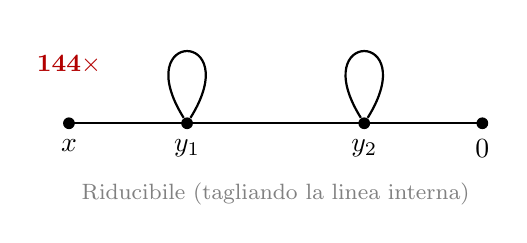
\begin{tikzpicture}[scale=1.5, 
        vertex/.style={circle, fill=black, inner sep=1.5pt},
        label_node/.style={font=\small},
        multiplicity/.style={font=\small\bfseries, color=red!70!black}
    ]
    \begin{scope}[shift={(0,0)}]
        
        
        % Linea di base
        \draw[thick] (0,0) -- (3.5,0);
        
        % Vertici
        \node[vertex, label=below:$x$] (x) at (0,0) {};
        \node[vertex, label=below:$y_1$] (y1) at (1,0) {};
        \node[vertex, label=below:$y_2$] (y2) at (2.5,0) {};
        \node[vertex, label=below:$0$] (z) at (3.5,0) {};
        
        % Loops (Bools)
        \draw[thick] (y1) .. controls (0.5, 0.8) and (1.5, 0.8) .. (y1);
        \draw[thick] (y2) .. controls (2.0, 0.8) and (3.0, 0.8) .. (y2);
        
        % Molteplicità
        \node[multiplicity] at (0, 0.5) {$\mathbf{144 \times}$};
        
        % Nota sotto
        \node[font=\footnotesize, color=gray] at (1.75, -0.6) {Riducibile (tagliando la linea interna)};
    \end{scope}
    \end{tikzpicture}
    \end{center}

    \item \textbf{Il "Setting Sun" (o "Hamburger"):}
    Partiamo da $x$ a $y_1$, e da $y_1$ a $y_2$ abbiamo 3 linee distinte, poi da $y_2$ a $0$.
   
    \begin{itemize}
        \item Contrarre $\varphi(x)$ con $y_1$, $\varphi(0)$ con $y_2$. Connettere $y_1$ e $y_2$ con 3 propagatori.
        \item Fattore combinatorio: $96$.
        \item Valore proporzionale a: $G_0(x-y_1) G_0(y_1-y_2)^3 G_0(y_2)$.
    \end{itemize}

    % --- DIAGRAMMA 2: Setting Sun ---
    \begin{center}
    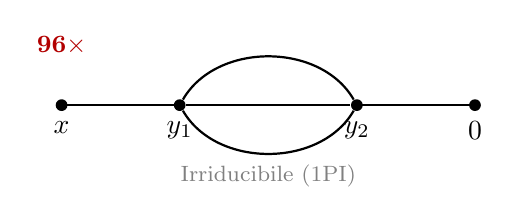
\begin{tikzpicture}[scale=1.5, 
        vertex/.style={circle, fill=black, inner sep=1.5pt},
        label_node/.style={font=\small},
        multiplicity/.style={font=\small\bfseries, color=red!70!black}
    ]
    \begin{scope}[shift={(0,0)}]
      
        % Gambe esterne
        \draw[thick] (0,0) -- (1,0); 
        \draw[thick] (2.5,0) -- (3.5,0); 
        
        % Vertici
        \node[vertex, label=below:$x$] (x) at (0,0) {};
        \node[vertex, label=below:$y_1$] (y1) at (1,0) {};
        \node[vertex, label=below:$y_2$] (y2) at (2.5,0) {};
        \node[vertex, label=below:$0$] (z) at (3.5,0) {};
        
        % 3 Linee interne (Tramonto)
        \draw[thick] (y1) -- (y2);                 % linea centrale
        \draw[thick] (y1) to[bend left=60] (y2);   % arco sopra
        \draw[thick] (y1) to[bend right=60] (y2);  % arco sotto
        
        % Molteplicità
        \node[multiplicity] at (0, 0.5) {$\mathbf{96 \times}$};
        
        % Nota sotto
        \node[font=\footnotesize, color=gray] at (1.75, -0.6) {Irriducibile (1PI)};
    \end{scope}
    \end{tikzpicture}
    \end{center}

    \item \textbf{La "Figura a Otto":}
    Due tadpoles connessi da una linea, in una variazione simmetrica.
   
    \begin{itemize}
        \item Fattore combinatorio: $144$.
        \item Valore proporzionale a: $G_0(x-y_1)G_0(y_2) G_0(y_1-y_2) G_0^2(0)$.
    \end{itemize}

    % --- DIAGRAMMA 3: Cactus ---
    \begin{center}
    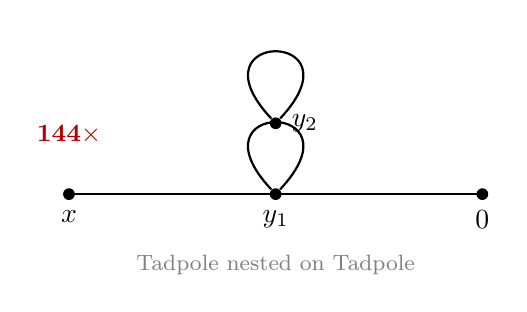
\begin{tikzpicture}[scale=1.5, 
        vertex/.style={circle, fill=black, inner sep=1.5pt},
        label_node/.style={font=\small},
        multiplicity/.style={font=\small\bfseries, color=red!70!black}
    ]
    \begin{scope}[shift={(0,0)}]
        
        
        % Linea di base continua
        \draw[thick] (0,0) -- (3.5,0);
        
        % Vertici
        \node[vertex, label=below:$x$] (x) at (0,0) {};
        \node[vertex, label=below:$y_1$] (y1) at (1.75,0) {}; 
        \node[vertex, label=below:$0$] (z) at (3.5,0) {};
        
        % Primo Loop (inferiore)
        \draw[thick] (y1) .. controls (1.0, 0.8) and (2.5, 0.8) .. (y1);
        
        % Vertice intermedio y2
        \coordinate (apex) at (1.75, 0.6); 
        \node[vertex, label=right:$y_2$] (y2) at (apex) {};
        
        % Secondo Loop (superiore)
        \draw[thick] (y2) .. controls (1.0, 1.4) and (2.5, 1.4) .. (y2);
        
        % Molteplicità
        \node[multiplicity] at (0, 0.5) {$\mathbf{144 \times}$};
        
        % Nota sotto
        \node[font=\footnotesize, color=gray] at (1.75, -0.6) {Tadpole nested on Tadpole};
    \end{scope}
    \end{tikzpicture}
    \end{center}
\end{enumerate}

\subsection{Riepilogo della Procedura }

Per calcolare la funzione di correlazione a qualsiasi ordine:

\begin{enumerate}
    \item Disegnare tutti i diagrammi di Feynman \textbf{connessi} topologicamente distinti con 2 punti esterni ($x$ e $0$) e $n$ vertici.
   
    \item I vertici hanno valenza 4 (4 linee che si incontrano).
    \item Assegnare un fattore $G_0(z_i - z_j)$ a ciascuna linea.
   
    \item Assegnare un fattore $(-g)$ a ciascun vertice (e i fattoriali appropriati dall'espansione).
   
    \item Moltiplicare per il \textbf{fattore combinatorio} (molteplicità) del diagramma.
    Questo conta il numero di modi per contrarre i campi per formare quella specifica topologia.
   
    \item Integrare sulle posizioni di tutti i vertici interni $y_1, \dots, y_n$.
   
\end{enumerate}

La cancellazione dei diagrammi disconnessi (vacuum bubbles)) assicura che la densità di energia libera e le funzioni di correlazione rimangano ben definite.